\documentclass[conference]{IEEEtran}
% \IEEEoverridecommandlockouts  % only needed if citing a funding source in \thanks{}

\usepackage{cite}
\usepackage{amsmath,amssymb,amsfonts}
\usepackage{graphicx}
\usepackage{textcomp}
\usepackage{xcolor}
\usepackage{booktabs}
\usepackage{multirow}

\def\BibTeX{{\rm B\kern-.05em{\sc i\kern-.025em b}\kern-.08em
    T\kern-.1667em\lower.7ex\hbox{E}\kern-.125emX}}

\begin{document}

\title{Intelligent Student Performance Analytics and\\Learning Strategy Optimization:\\A Multi-Dataset Data Mining Approach}

\author{
  \IEEEauthorblockN{Nadugala Vithanage Yasitha Priyashan}
  \IEEEauthorblockA{
    \textit{Department of Computer Science \& Engineering} \\
    \textit{University of Moratuwa} \\
    Moratuwa, Sri Lanka \\
    Priyashann.26@cse.mrt.ac.lk
  }
}

\maketitle

\begin{abstract}
Early identification of struggling students remains a critical challenge in educational environments. This study applies data mining techniques to three complementary educational datasets — the UCI Student Performance Dataset (Mathematics, 395 students), the UCI Student Performance Dataset (Portuguese Language, 649 students), and the xAPI Behavioral Education Dataset (478 students) — to identify patterns in student achievement and propose actionable strategies for academic improvement. We perform exploratory data analysis, build three supervised classifiers (two Random Forest models for pass/fail prediction and one Gradient Boosting classifier for three-class performance prediction), apply K-Means clustering to uncover distinct learner profiles, and mine association rules to surface behavioral patterns linked to academic outcomes. Our Random Forest models achieve \textbf{86.08\%} accuracy (AUC = 0.9419) on Math and \textbf{87.69\%} (AUC = 0.9373) on Portuguese pass/fail prediction, while the Gradient Boosting classifier reaches \textbf{76.04\%} accuracy across three performance levels. A notable cross-subject finding is that Portuguese grades average 2.13 points higher than Math grades for the same students (paired $t$-test $p < 10^{-20}$), with a moderate correlation of $r = 0.48$ between subjects. Clustering reveals three learner archetypes — \textit{Active}, \textit{Moderate}, and \textit{Passive} — that closely align with actual class outcomes. The findings suggest that behavioral engagement and early academic performance are the strongest predictors of final outcomes, with direct implications for early-warning systems and targeted intervention design.
\end{abstract}

\begin{IEEEkeywords}
student performance prediction, educational data mining, learning analytics, classification, clustering, association rules, xAPI, UCI dataset
\end{IEEEkeywords}

\noindent\textit{Revised version, September 2026. This revision corrects errors found in the original submission (April 2026); all changes are listed in the Appendix. Code and data: \texttt{github.com/YasithaNV2001/student-performance-analytics}.}

% ─────────────────────────────────────────────────────────────────────────────
\section{Introduction}

Educational institutions generate an enormous volume of student data — grades, attendance records, behavioral logs, and demographic details — yet much of this information sits unused when it comes to identifying at-risk students early or personalizing the learning experience. The field of Educational Data Mining (EDM) aims to change that, using computational techniques to extract meaningful patterns from these data sources \cite{romero2010educational}.

Timely intervention is critical; delayed identification of at-risk students negatively impacts final academic outcomes \cite{baker2010data}. Understanding the behavioral and social factors associated with academic performance can further inform curriculum design, advising strategies, and resource allocation.

This study evaluates student performance through two distinct data perspectives. First, we use the UCI Student Performance Dataset \cite{cortez2008using}, which captures final grades alongside rich demographic and social variables for secondary school students in Portugal — separately for Mathematics (395 students) and Portuguese Language (649 students). Analyzing both subjects for the same population of 382 dual-enrolled students allows us to investigate whether risk factors are subject-specific or reflect broader student characteristics. Second, we incorporate the xAPI-Edu-Data \cite{amrieh2016mining}, which tracks behavioral engagement — specifically how often students raise hands, visit learning resources, view announcements, and participate in discussions. Together, these three datasets allow us to examine both \textit{what students do} and \textit{how they perform}, giving us a more complete picture than any single dataset could provide.

Our analysis has three main goals: (1) build predictive models that can flag at-risk students early, (2) discover natural groupings of students based on behavioral engagement, and (3) identify association rules connecting behavioral patterns to academic outcomes. The insights from each thread are synthesized into a set of practical recommendations for educators and institutions.

The rest of this paper is organized as follows. Section II reviews related work. Section III describes the datasets and preprocessing steps. Section IV presents our methodology. Section V reports results. Section VI discusses the findings and their implications. Section VII concludes the paper.

% ─────────────────────────────────────────────────────────────────────────────
\section{Related Work}

Educational data mining is a well-established research area. Romero and Ventura \cite{romero2010educational} provide a comprehensive survey of methods and applications, covering everything from association rule mining of course interactions to neural network-based grade prediction. Their review highlights that most studies focus on either predicting grades or identifying at-risk students, but rarely both within a unified framework.

Cortez and Silva \cite{cortez2008using} introduced the UCI Student Performance Dataset and demonstrated that Decision Trees, Random Forests, and Neural Networks could predict binary pass/fail outcomes with reasonable accuracy using demographic and social features. They found that the number of past course failures and parental education level were among the most predictive features — a finding we revisit and extend to both Mathematics and Portuguese Language in our own analysis.

Amrieh et al.~\cite{amrieh2016mining} analyzed the xAPI dataset using Naive Bayes, Decision Trees, and Neural Networks, achieving accuracy values between 73\% and 79\% for three-class classification (Low, Medium, High). They emphasized the importance of student-initiated behaviors — particularly raising hands and visiting resources — as stronger predictors than passive indicators like announcement views. Our Gradient Boosting model achieves 76.04\% accuracy on the same task, consistent with their reported range.

More recent work has moved toward combining behavioral signals with academic records. Hlosta et al.~\cite{hlosta2017ouroboros} used the Open University Learning Analytics Dataset (OULAD) to build an early warning system, demonstrating that engagement features in the first few weeks of a course are predictive of final outcomes weeks or months later. This supports the intuition that what students do early on sets the trajectory for where they end up.

Our work contributes to this body of knowledge by applying a consistent analytical pipeline — supervised classification, unsupervised clustering, and association rule mining — across three distinct educational datasets, enabling both within-dataset and cross-dataset validation of findings.

% ─────────────────────────────────────────────────────────────────────────────
\section{Data Description and Preparation}

\subsection{Datasets}

We use three datasets in this study:

\textbf{UCI Student Performance — Mathematics} \cite{cortez2008using}: Records for 395 secondary school students in Portugal covering the mathematics course. Features include demographic attributes (age, sex, address), family background (parental education and occupation, family size), social habits (alcohol consumption, going-out frequency, romantic relationships), and school-related variables (study time, absences, extra support, past failures). The primary outcome is the final grade G3 (0–20 scale). Pass threshold: G3~$\geq$~10 (67.1\% pass rate).

\textbf{UCI Student Performance — Portuguese Language} \cite{cortez2008using}: Records for 649 students from the same schools with an identical 33-column structure. Pass threshold: G3~$\geq$~10 (84.6\% pass rate — 17.5 percentage points higher than Math). Of these students, 382 are dual-enrolled in both courses, enabling direct cross-subject comparison.

\textbf{xAPI-Edu-Data} \cite{amrieh2016mining}: Records for 480 students (478 after removing two duplicate rows) across multiple educational levels, capturing four behavioral interaction counts (raised hands, resources visited, announcements viewed, discussion posts), demographic features (gender, nationality, stage, topic, semester), and parental involvement indicators. The outcome is a three-class label: Low (L, 26.2\%), Medium (M, 44.1\%), and High (H, 29.7\%) performance.

\subsection{Preprocessing}

Neither dataset contained missing values, which simplified the preparation process. Raw data quality was audited before cleaning — confirming zero missing values in all three datasets and zero duplicate rows in both UCI datasets. The xAPI dataset contained two duplicate rows, which were removed. For the UCI datasets, we applied label encoding to categorical features (sex, address, family size, parental job categories, and binary yes/no variables). For xAPI, we similarly encoded binary columns (gender, semester, parental survey response, school satisfaction, absence level). Cleaned datasets were saved to disk and reloaded to confirm reproducibility.

\subsection{Feature Engineering}

We derived several additional features to enrich the analysis:

\begin{itemize}
  \item \textbf{Grade trend} (UCI): G2 $-$ G1, capturing whether a student's performance is improving or declining.
  \item \textbf{Average alcohol consumption} (UCI): Mean of weekday (Dalc) and weekend (Walc) alcohol scores.
  \item \textbf{Parental education average} (UCI): Mean of maternal (Medu) and paternal (Fedu) education levels.
  \item \textbf{Study-absence ratio} (UCI): Study time $\div$ (absences + 1), capturing the balance between effort and attendance.
  \item \textbf{Composite engagement score} (xAPI): Mean of all four behavioral interaction counts, providing a single summary of overall engagement.
  \item \textbf{High-absence flag} (xAPI): Binary indicator for students with above-7 absences.
\end{itemize}

These engineered features consistently appeared among the top predictors in our models (see Section~\ref{sec:results}).

% ─────────────────────────────────────────────────────────────────────────────
\section{Methodology}

Our analysis follows four sequential steps, illustrated in Fig.~\ref{fig:pipeline}.

\begin{figure}[htbp]
  \centering
  \framebox{\parbox{0.9\columnwidth}{\centering\small
    Data Loading \& Cleaning $\rightarrow$ EDA \& Feature Engineering \\[4pt]
    $\downarrow$ \\[2pt]
    Supervised Classification (RF $\times$2 + GB) \\[4pt]
    $\downarrow$ \\[2pt]
    Unsupervised Clustering (K-Means $\times$2) \\[4pt]
    $\downarrow$ \\[2pt]
    Association Rule Mining (Apriori $\times$2)
  }}
  \caption{Overall analysis pipeline.}
  \label{fig:pipeline}
\end{figure}

\subsection{Supervised Learning}

\textbf{Models 1 \& 2 — Random Forest (UCI Pass/Fail):} We trained Random Forest classifiers with 300 trees (max depth = 10, min samples per leaf = 3) to predict whether a student would pass or fail (binary). One model was trained per subject (Math and Portuguese) to compare predictability across courses. The training/test split was 80/20 with stratification, and we used 5-fold cross-validation to estimate generalization performance. Class imbalance was addressed through \texttt{class\_weight='balanced'}.

\textbf{Model 3 — Gradient Boosting (xAPI Multi-class):} For the three-class prediction task on the xAPI dataset, we used a Gradient Boosting Classifier with 200 estimators, a learning rate of 0.08, maximum tree depth of 4, and subsample ratio of 0.8. The same 80/20 stratified split and 5-fold cross-validation strategy were applied.

All models were evaluated using accuracy, macro-averaged AUC-ROC, and detailed classification reports including precision, recall, and F1-score per class.

\subsection{Unsupervised Clustering}

K-Means clustering was applied to both the UCI (Math + Portuguese combined) and xAPI behavioral features after standardization (zero mean, unit variance). We selected $k$ by examining both the elbow curve of inertia values and silhouette scores for $k \in \{2, \ldots, 8\}$. The resulting clusters were projected to two dimensions using PCA for visualization and profiled by mean feature values to assign descriptive learner archetypes.

\subsection{Association Rule Mining}

We applied the Apriori algorithm \cite{agrawal1994fast} to binarized versions of both datasets. Continuous behavioral features were discretized at their median values into ``high'' and ``low'' binary flags. Rules were mined with minimum support of 0.12 (xAPI) and 0.10 (UCI), and ranked by lift to surface the most informative patterns.

% ─────────────────────────────────────────────────────────────────────────────
\section{Results}
\label{sec:results}

\subsection{Exploratory Data Analysis}

Grade distributions in the UCI dataset show a roughly normal shape centered around 10–12, with a noticeable spike at zero — likely students who withdrew or were absent for the final assessment. Pass rates differ substantially between subjects (67.1\% Math vs.\ 84.6\% Portuguese). For the 382 dual-enrolled students, a paired $t$-test confirms that Portuguese grades are significantly higher than Math grades by an average of 2.13 points ($t = -9.98$, $p = 5.56 \times 10^{-21}$), with a moderate correlation of $r = 0.480$ ($p < 0.001$) between the two subjects.

Fig.~\ref{fig:grades} shows the grade distributions for each period. The spike at zero appears mainly in the final grade (G3), and is larger for Math than for Portuguese.

\begin{figure}[htbp]
  \centering
  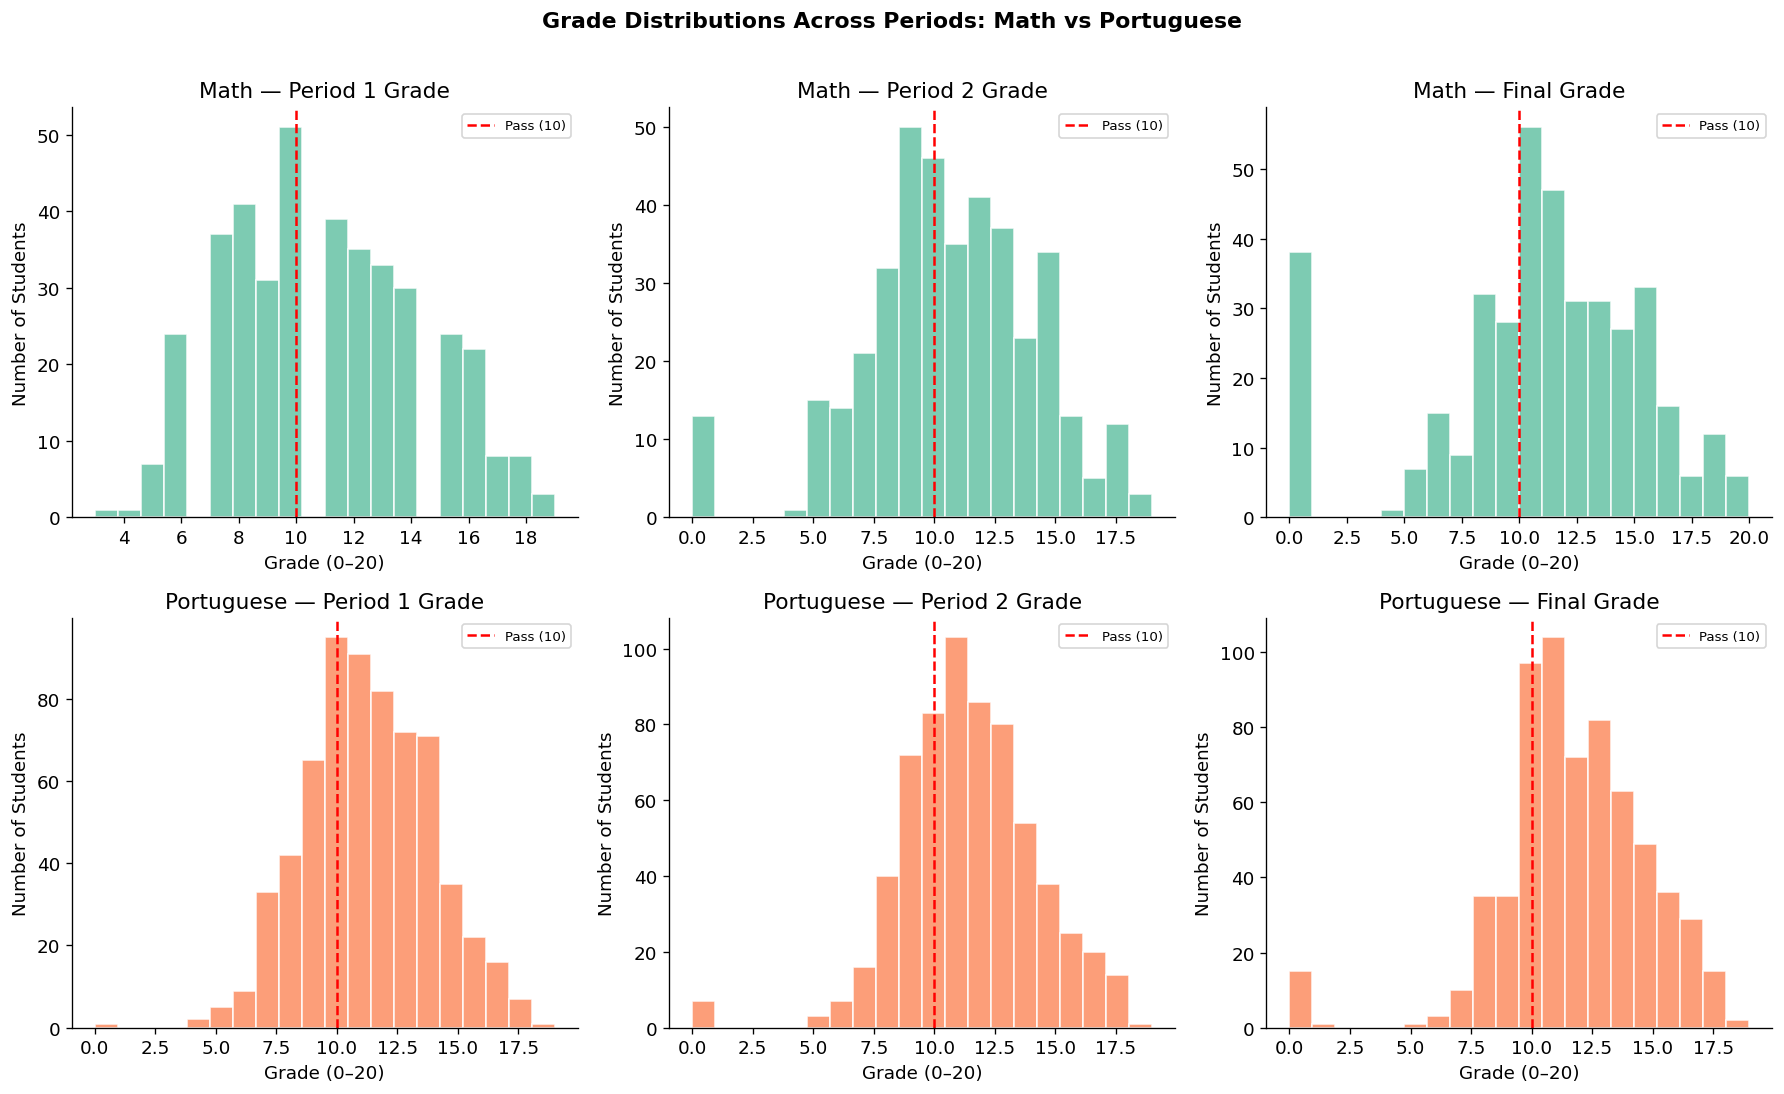
\includegraphics[width=\columnwidth]{report_figures/fig2_pass_factors.png}
  \caption{Grade distributions for the first period (G1), second period (G2) and final grade (G3), for Math (top) and Portuguese (bottom). The dashed line marks the pass threshold of 10.}
  \label{fig:grades}
\end{figure}

The correlation heatmap (Fig.~\ref{fig:corr}) confirms that G1 and G2 are strongly correlated with G3 ($r > 0.80$), while past failures show a moderate negative correlation ($r = -0.36$ Math, $-0.39$ Portuguese). Absences show almost no linear relationship with G3 ($r = 0.03$ Math, $-0.09$ Portuguese). Weekday and weekend alcohol consumption are weakly negatively correlated with G3 in Portuguese ($r = -0.20$ and $-0.18$), but not in Math ($r = -0.05$).

\begin{figure}[htbp]
  \centering
  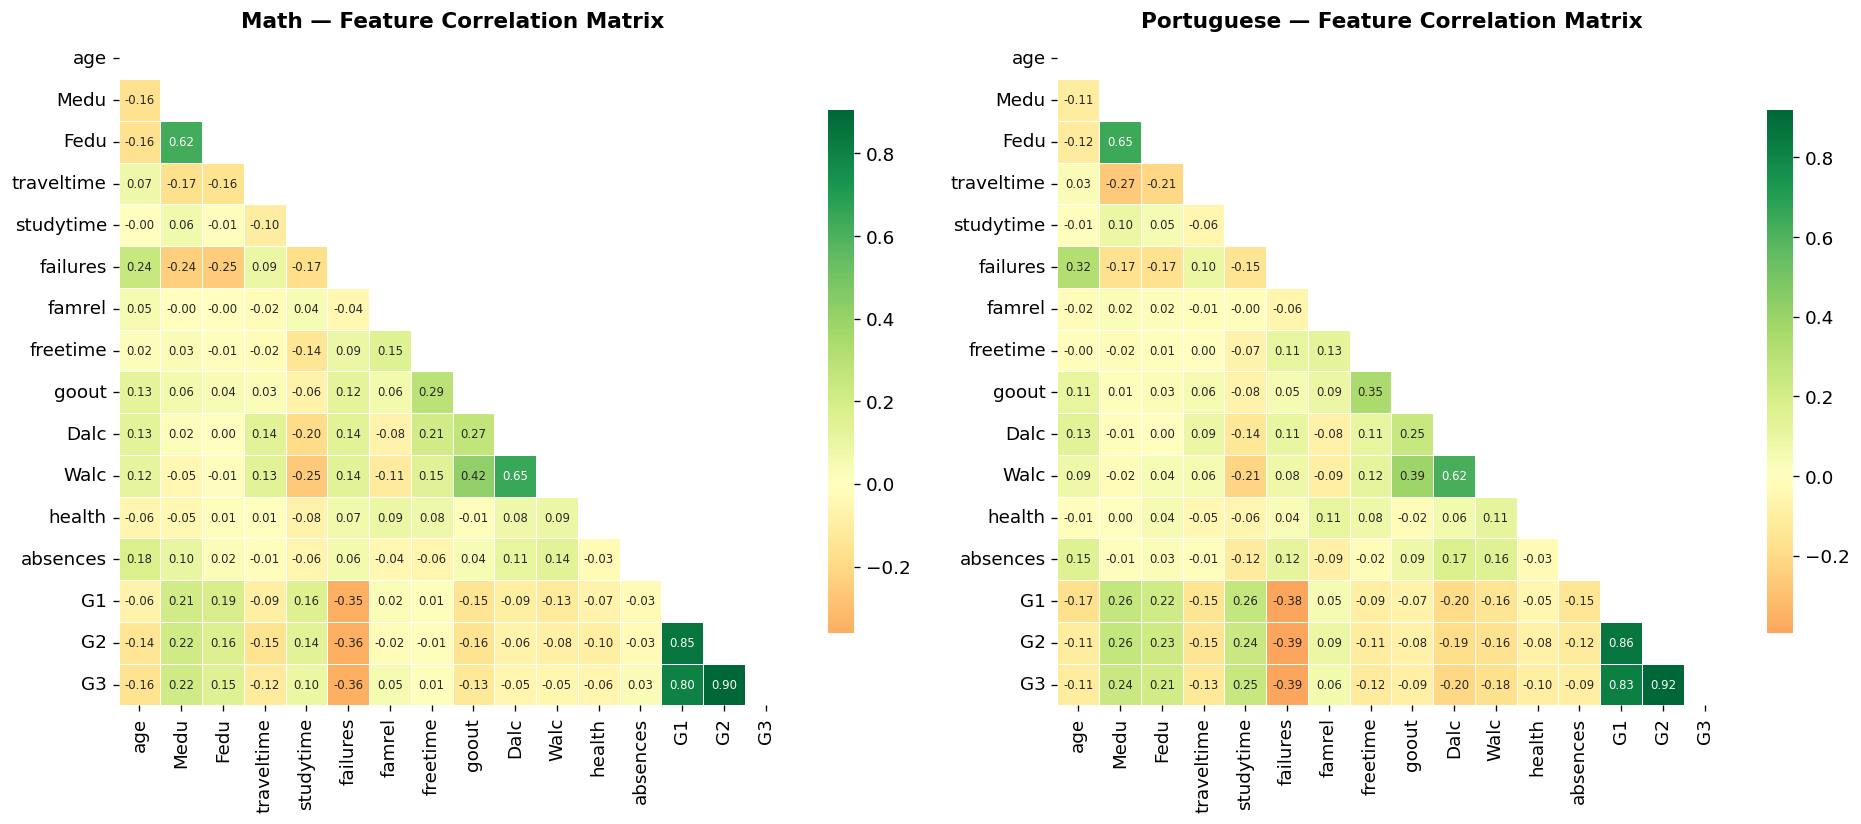
\includegraphics[width=\columnwidth]{report_figures/fig3_correlation.png}
  \caption{Pearson correlation matrices for UCI numeric features, Math (left) and Portuguese (right). Green indicates positive and orange negative correlations.}
  \label{fig:corr}
\end{figure}

For the xAPI dataset, behavioral engagement levels differ sharply between performance classes. High-performing students raised their hands about four times as often as low-performing students on average (4.2$\times$), and their resource visit counts were similarly elevated (Fig.~\ref{fig:engagement}). A Kruskal-Wallis test confirms the engagement score distributions are significantly different across all three classes ($H = 239.0$, $p < 10^{-50}$).

\begin{figure}[htbp]
  \centering
  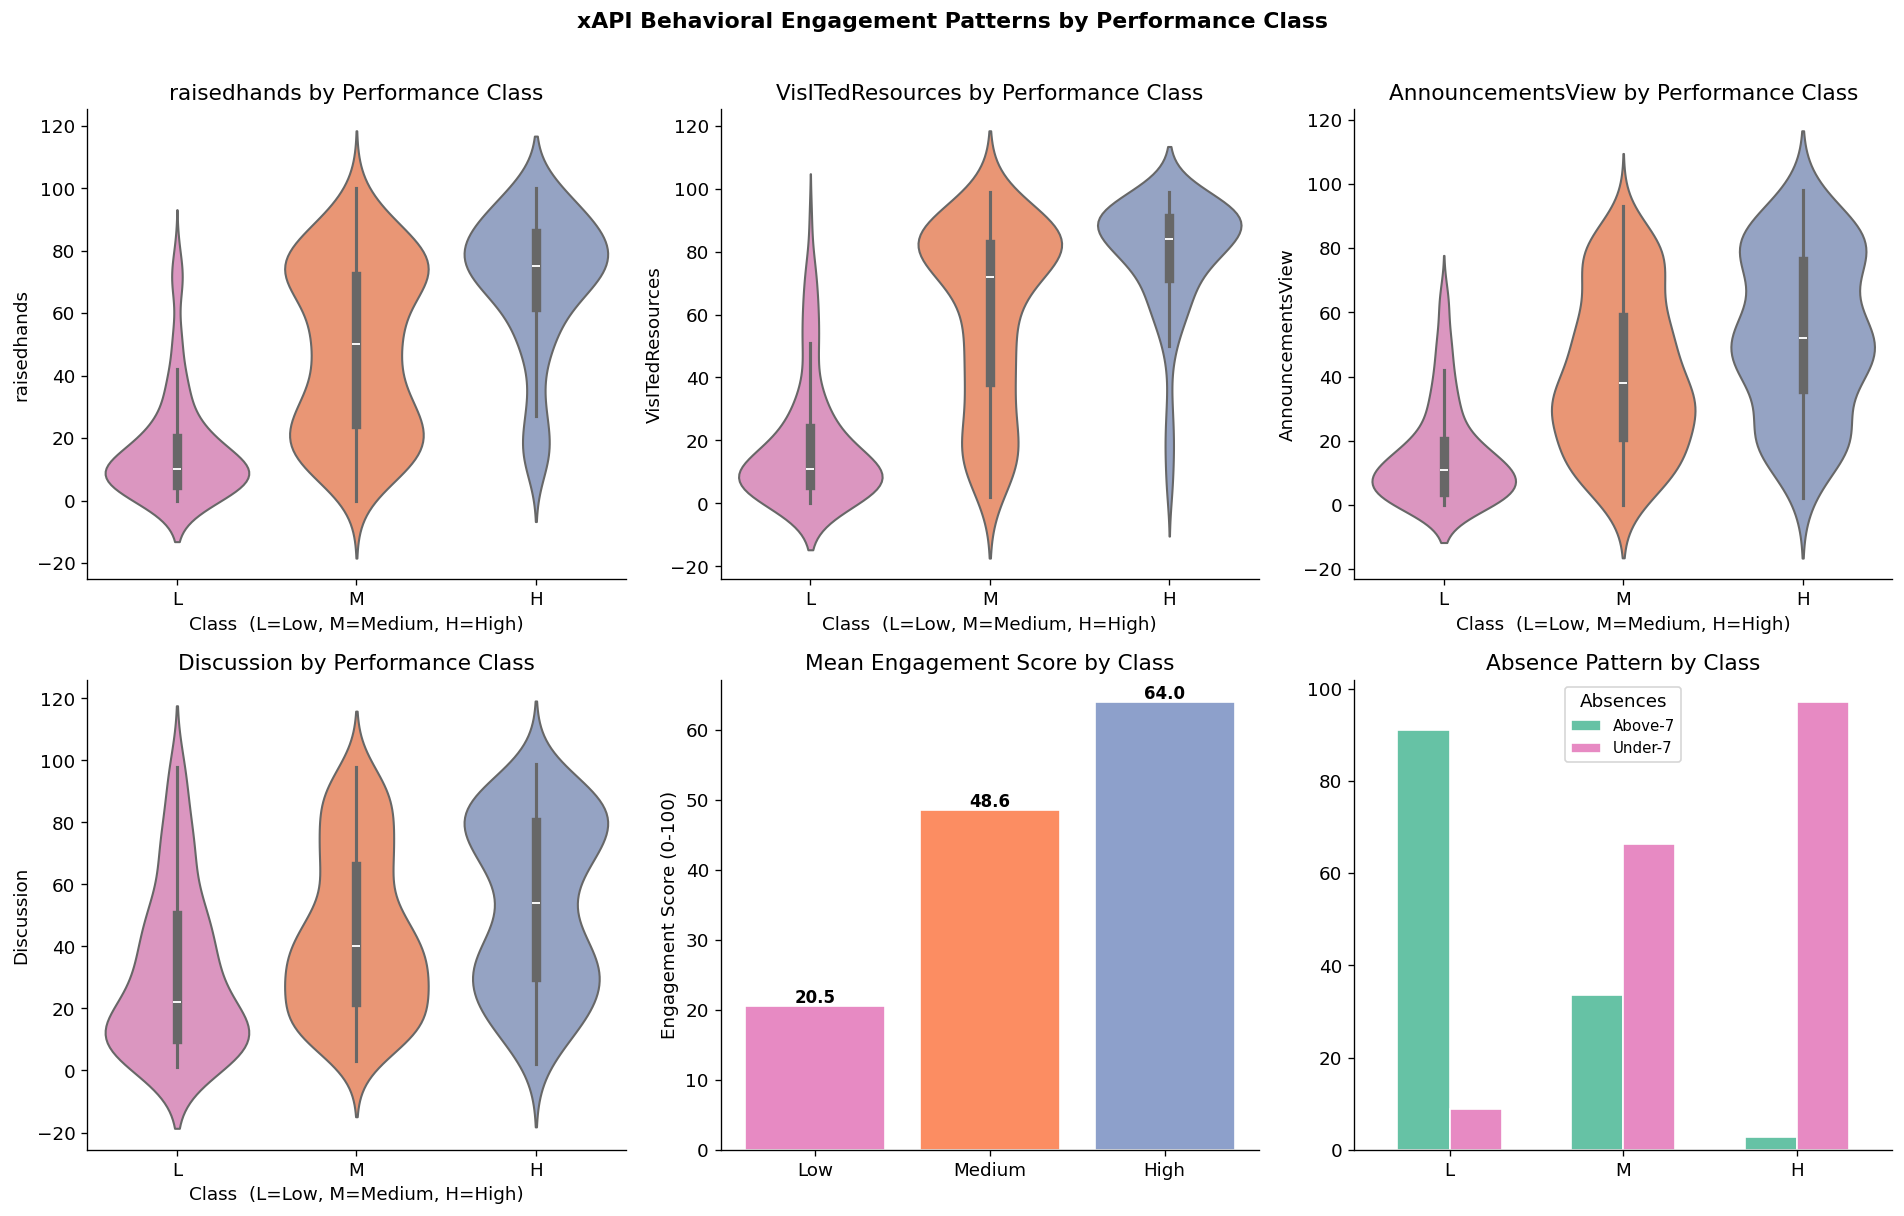
\includegraphics[width=\columnwidth]{report_figures/fig4_engagement.png}
  \caption{Engagement score distributions and absence patterns by performance class (xAPI dataset). The High class shows both higher engagement and lower absence rates.}
  \label{fig:engagement}
\end{figure}

\subsection{Supervised Classification Results}

Table~\ref{tab:models} summarizes the performance of all three classifiers.

\begin{table}[htbp]
  \centering
  \caption{Supervised Model Performance Comparison}
  \label{tab:models}
  \setlength{\tabcolsep}{4pt}
  \begin{tabular}{llccc}
    \toprule
    \textbf{Model} & \textbf{Dataset} & \textbf{Acc. (\%)} & \textbf{AUC} & \textbf{CV Acc. (\%)} \\
    \midrule
    RF & Math       & 86.08 & 0.9419 & 90.63 $\pm$ 2.35 \\
    RF & Portuguese & 87.69 & 0.9373 & 92.45 $\pm$ 0.90 \\
    GB & xAPI       & 76.04 & 0.9175 & 74.89 $\pm$ 6.50 \\
    \bottomrule
  \end{tabular}

  \vspace{2pt}
  {\footnotesize RF = Random Forest (binary pass/fail); GB = Gradient Boosting (3-class). CV = 5-fold cross-validation, mean $\pm$ std.}
\end{table}

The Random Forest classifiers perform well on both binary tasks. The confusion matrix in Fig.~\ref{fig:rf_results} shows relatively few false negatives — a desirable property for an early-warning system, since it is preferable to flag a student who turns out to be fine than to miss one who is genuinely at risk. The higher variance in xAPI cross-validation (±6.50\%) compared to UCI (±0.90–2.35\%) reflects both the smaller sample size and the three-class task difficulty.

\begin{figure}[htbp]
  \centering
  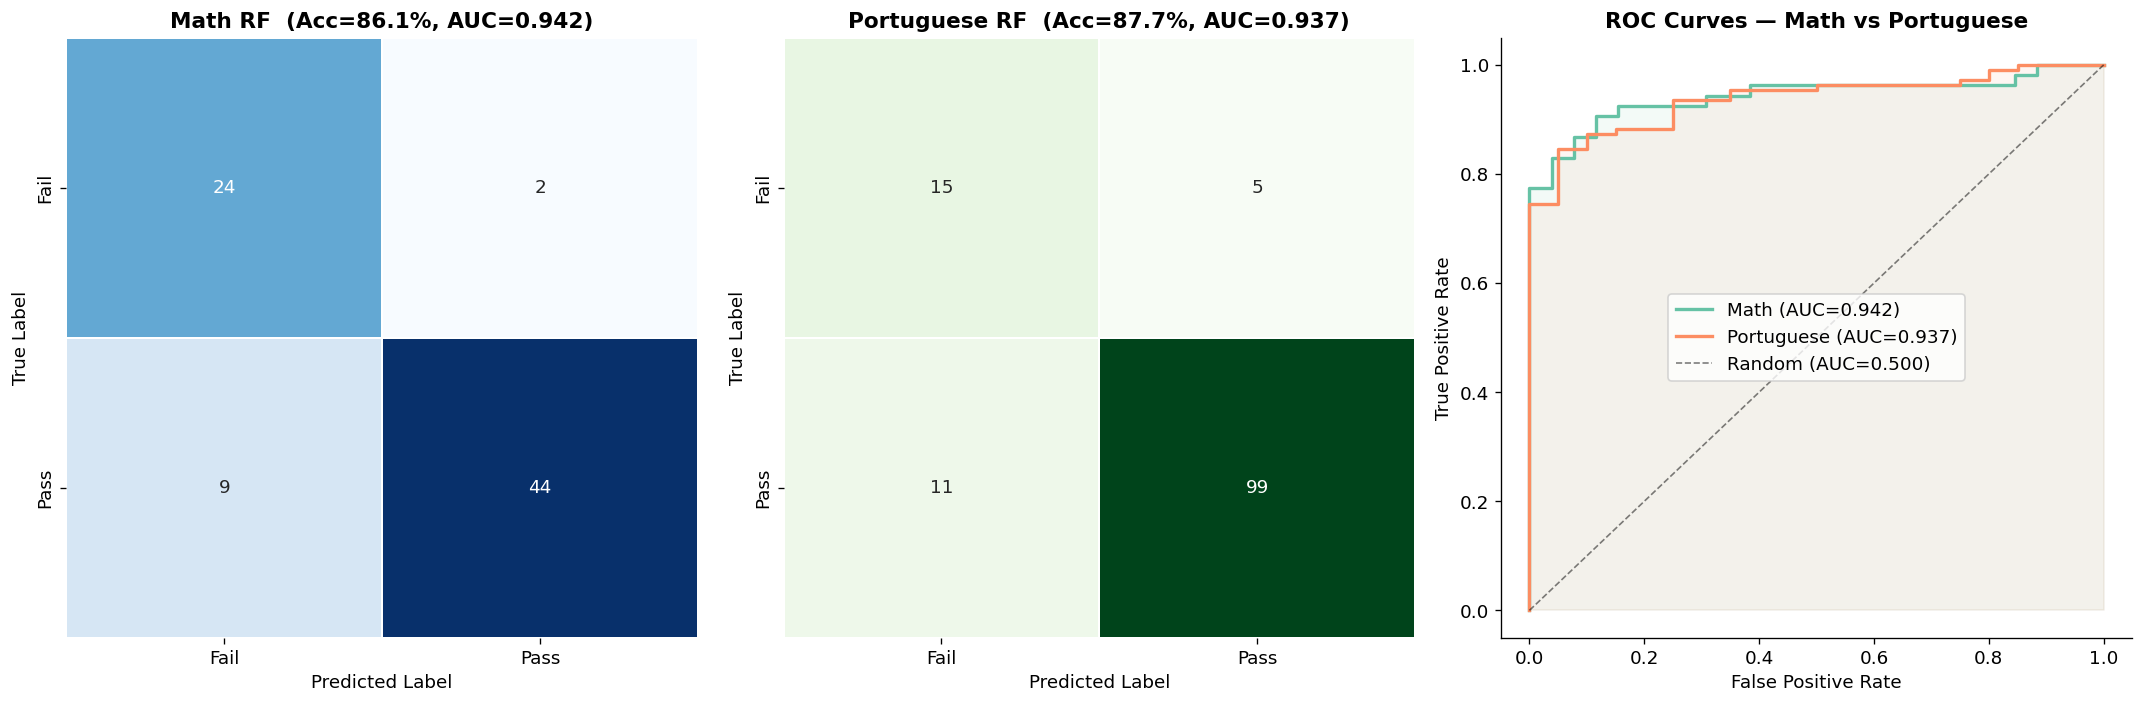
\includegraphics[width=\columnwidth]{report_figures/fig5_rf_results.png}
  \caption{Random Forest performance: confusion matrices for the Math (left) and Portuguese (center) models, and ROC curves for both (right).}
  \label{fig:rf_results}
\end{figure}

Fig.~\ref{fig:model_comparison} summarizes accuracy and AUC-ROC across all three classifiers. All models exceed 0.91 AUC, indicating strong discriminative ability regardless of dataset or task type. The Random Forest models are notably more stable than Gradient Boosting (CV variance ±0.90–2.35\% vs.\ ±6.50\%), which is consistent with the smaller xAPI sample size and the added complexity of three-class prediction.

\begin{figure}[htbp]
  \centering
  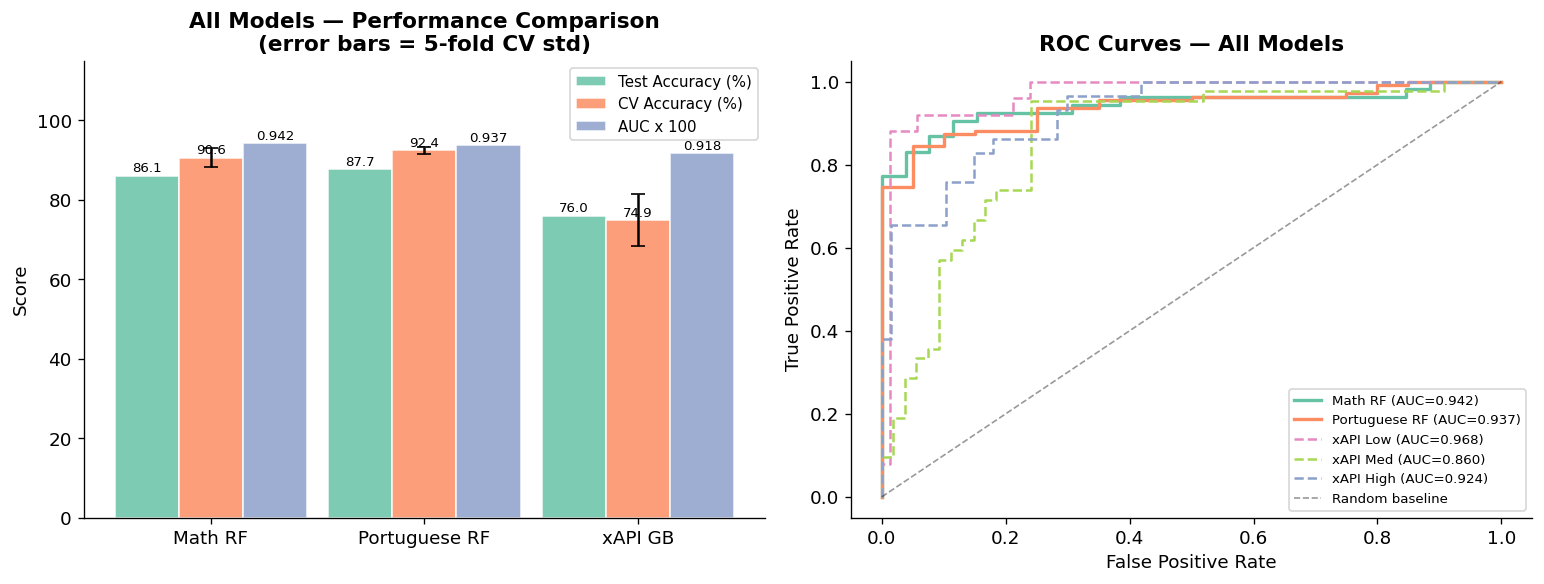
\includegraphics[width=\columnwidth]{report_figures/fig6_model_comparison.png}
  \caption{Model performance summary across all three classifiers. AUC-ROC scores above 0.91 for all models indicate strong discriminative ability.}
  \label{fig:model_comparison}
\end{figure}

Feature importance analysis reveals that the second-period grade (G2, $r = 0.905$) is the strongest predictor of final outcome, followed by G1 ($r = 0.801$) and past failures ($r = -0.360$). The engineered grade trend feature also appears in the top ten, indicating that trajectory matters beyond absolute grade level. For the xAPI dataset, the composite engagement score is the single most important feature, followed by raised hands and resources visited. Parental involvement (survey response) ranks fourth, echoing findings on family support in academic outcomes \cite{fan1998parental}.

\subsection{Clustering Results}

Silhouette analysis supports $k = 3$ as the natural number of clusters for both datasets. Table~\ref{tab:clustering} summarizes the cluster evaluation metrics.

\begin{table}[htbp]
  \centering
  \caption{Clustering Evaluation Metrics ($k = 3$)}
  \label{tab:clustering}
  \begin{tabular}{lccc}
    \toprule
    \textbf{Dataset} & \textbf{Silhouette} & \textbf{Davies-Bouldin} & \textbf{Inertia} \\
    \midrule
    UCI (Math + Por.) & 0.190 & 1.686 & -- \\
    xAPI Behavioral   & 0.360 & 1.094 & -- \\
    \bottomrule
  \end{tabular}
  {\footnotesize Lower Davies-Bouldin is better (tighter, well-separated clusters).}
\end{table}

The lower silhouette score for UCI (0.190 vs.\ 0.360) reflects the continuum of academic performance rather than discrete groupings; behavioral data (xAPI) produces more compact, separable clusters, confirmed by its lower Davies-Bouldin score (1.094 vs.\ 1.686). The three clusters map onto interpretable learner archetypes:

\begin{itemize}
  \item \textbf{Active learners}: High engagement across all four behavioral dimensions, low absence rates, predominantly High-class students.
  \item \textbf{Moderate learners}: Middle-range engagement, mixed absence patterns, distributed across Medium and High classes.
  \item \textbf{Passive learners}: Low engagement, high absence rates, heavily concentrated in the Low class.
\end{itemize}

Fig.~\ref{fig:clustering} shows the PCA projection of the three clusters, which are largely separable in the reduced two-dimensional space.

\begin{figure}[htbp]
  \centering
  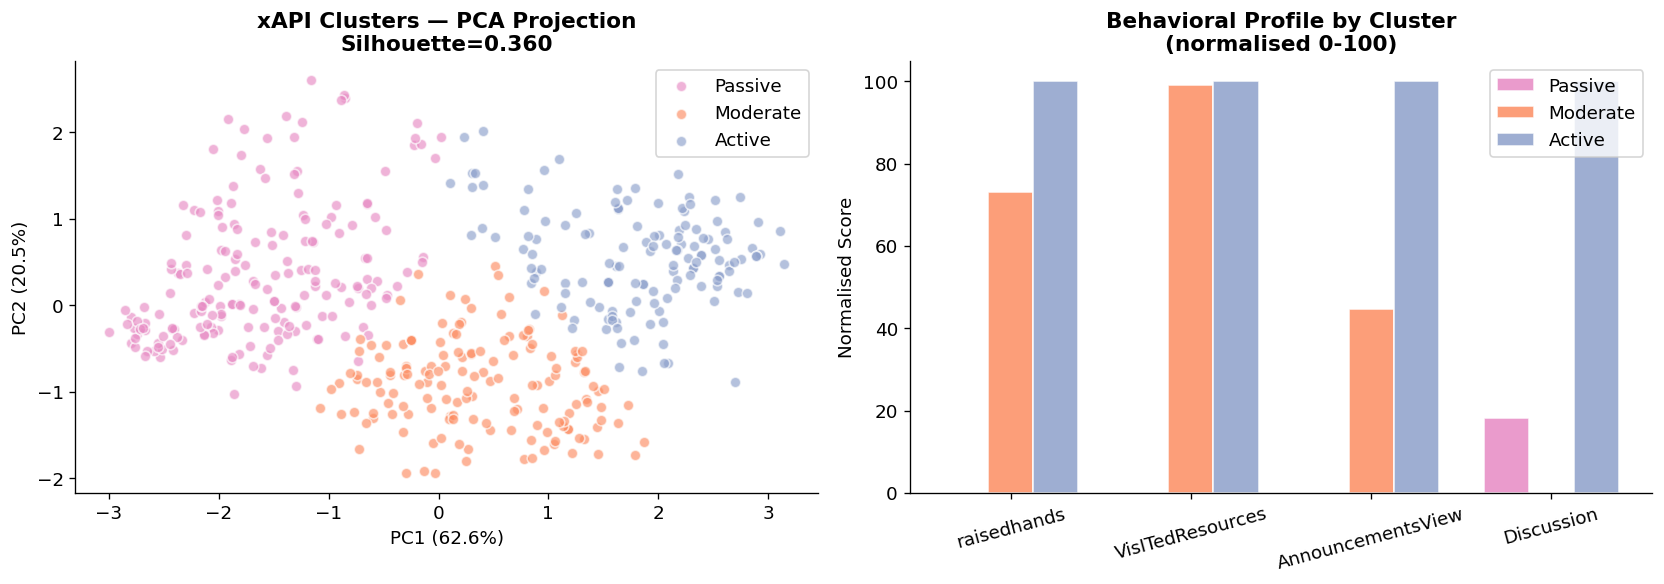
\includegraphics[width=\columnwidth]{report_figures/fig7_clustering.png}
  \caption{K-Means clustering of xAPI behavioral features ($k = 3$): PCA projection of the three clusters (left) and mean behavioral profile of each cluster, normalized to 0--100 (right). Silhouette score = 0.360.}
  \label{fig:clustering}
\end{figure}

\subsection{Association Rules}

The Apriori algorithm produces 11 class-predicting rules on the xAPI dataset and 25 pass/fail rules on the UCI dataset. Several rules stand out:

\begin{itemize}
  \item \textbf{xAPI best rule}: $\{\text{absent\_high}\} \Rightarrow \{\text{class\_low}\}$, confidence = 0.603, lift = 2.307.
  \item \textbf{UCI best rule}: $\{\text{alcohol\_high}, \text{failures\_any}\} \Rightarrow \{\text{fail}\}$, confidence = 0.678, lift = 2.060.
  \item Students with high raised-hands counts and high resource visits, combined with parental survey participation, are associated with the High class (confidence $\approx$ 0.58, lift $\approx$ 1.95).
  \item Parental engagement (answering the survey) combined with high announcement views predicts Medium or High class.
\end{itemize}

Fig.~\ref{fig:rules} plots the support-confidence relationship for the class-predicting rules, colored by lift. Rules in the upper-right region represent the most actionable patterns — both common and reliable.

\begin{figure}[htbp]
  \centering
  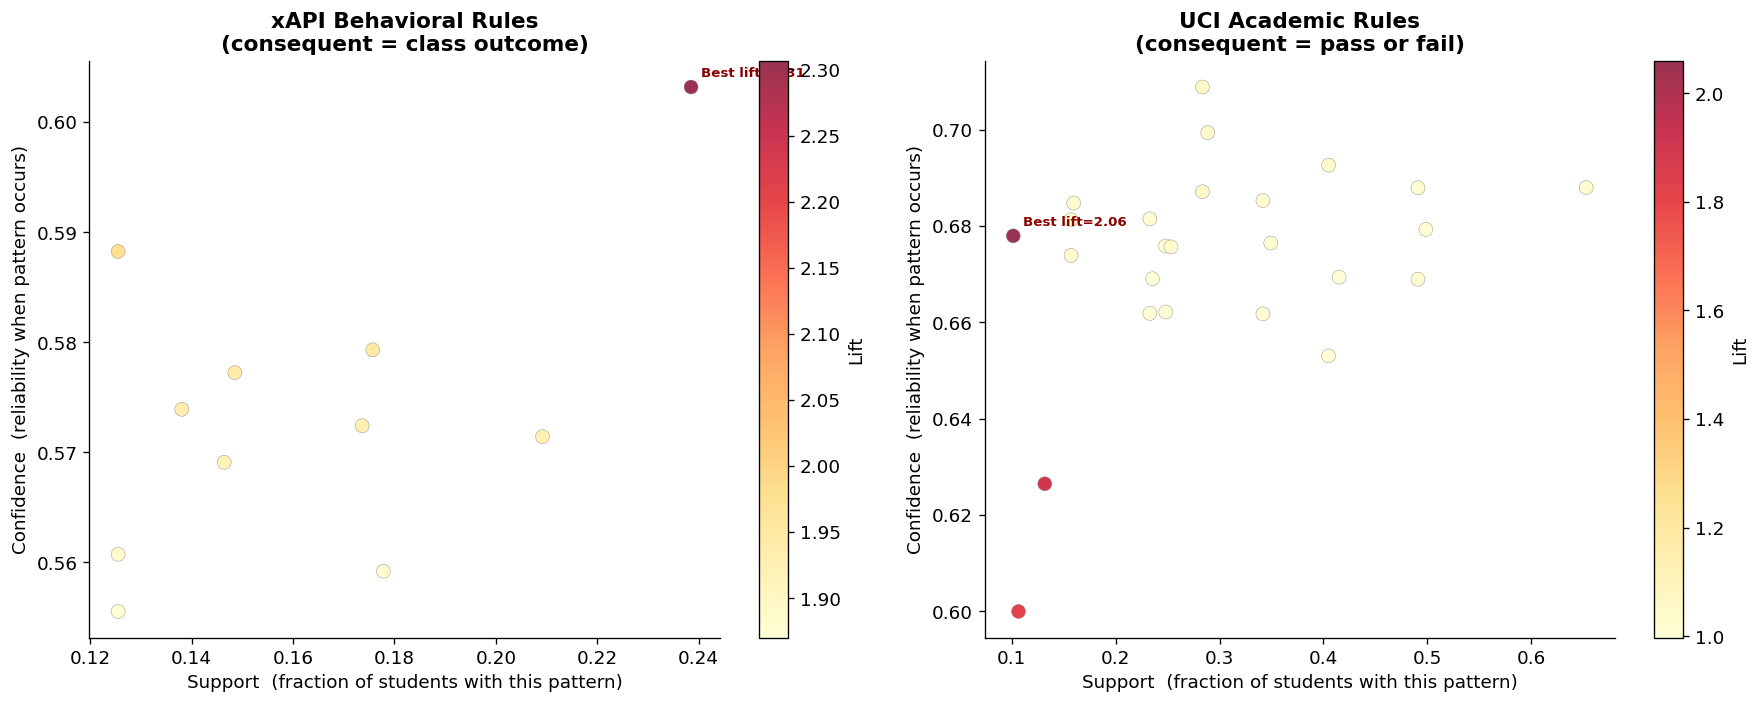
\includegraphics[width=\columnwidth]{report_figures/fig8_arm.png}
  \caption{Association rules scatter plot (support vs.\ confidence, colored by lift) for xAPI (left) and UCI (right). Rules in the upper-right quadrant are both frequent and reliable.}
  \label{fig:rules}
\end{figure}

% ─────────────────────────────────────────────────────────────────────────────
\section{Discussion}

\subsection{Key Findings}

The analytical pipeline demonstrates consistent predictive patterns across the three independent datasets. Academic history — particularly recent grades and past failures — dominates when predicting whether a student will pass or fail. This carries a practical implication: an early-warning system needs access to interim assessment data (like G2 in the UCI setting) to function well. Systems that rely only on demographic or social features at enrollment time will likely be far less accurate.

The cross-subject analysis adds a finding not captured in prior single-dataset studies: for the same 382 students, Portuguese grades are significantly higher than Math grades by 2.13 points on average, yet the two subjects correlate at $r = 0.480$. This means that a student's general academic capability partially transfers across subjects, but subject-specific factors (difficulty, teaching style, student motivation) also play a meaningful role. Risk models should account for this by being trained separately per subject rather than pooling grades across courses.

The behavioral findings from the xAPI analysis add a complementary layer. Even without grade history, how actively a student engages with course materials is strongly predictive of performance class. The association rules make this concrete: students with high absence combined with low engagement are very likely to end up in the Low category, while students showing the opposite pattern rarely do.

\subsection{Cross-Dataset Synthesis}

Although the three datasets cover different educational systems and cannot be directly merged, they tell a consistent story when analyzed side by side. Both point to the same root factors: effort (study time, raised hands, resource visits), consistency (absence levels, grade trends), and support structures (parental involvement, access to internet, family educational background). This convergence across independent datasets gives us more confidence in the recommendations that follow.

\subsection{Recommendations for Educators}

Based on our findings, we suggest the following:

\begin{enumerate}
  \item \textbf{Deploy early-warning systems as soon as interim grades are available.} G2 is the strongest predictor of final outcomes, but a follow-up analysis in the accompanying notebook shows that the first-period grade (G1) alone already recovers most of the predictive power (AUC 0.83--0.87). Schools should therefore flag students after the first grading period rather than waiting for G2.
  \item \textbf{Monitor engagement proxies in digital learning environments.} Resource visit counts and participation indicators from LMS platforms can serve as early signals of disengagement, even before grades reflect a problem.
  \item \textbf{Target passive learner clusters for proactive outreach.} The K-Means analysis identifies a cluster of low-engagement, high-absence students who are at high risk of poor outcomes.
  \item \textbf{Involve parents as part of the intervention strategy.} Both datasets suggest that parental engagement is a meaningful factor. Structured parent-school communication programs, particularly for at-risk students, may improve outcomes.
  \item \textbf{Build subject-specific risk models.} The significant grade gap and imperfect correlation between Math and Portuguese scores suggest that a single cross-subject model would obscure important subject-level variation.
\end{enumerate}

\subsection{Limitations}

Several limitations should be considered when interpreting these findings. First, the UCI dataset covers only two schools in Portugal in 2008, limiting geographic and temporal generalizability. Second, K-Means assumes spherical clusters of equal size — a strong assumption that the modest silhouette scores (0.19–0.36) suggest is only partially met. Third, the xAPI and UCI datasets cannot be directly merged because they cover different student populations, educational systems, and time periods; our cross-dataset synthesis is therefore inferential rather than confirmatory. Finally, the association rules reflect correlation, not causation — a rule such as \textit{absent\_high} $\Rightarrow$ \textit{class\_low} does not prove that attendance reduction causes poor performance; both may stem from an unmeasured confounding variable.

\subsection{Ethical Considerations}

Using student data to build predictive models raises genuine ethical questions. A model that predicts which students will fail can, if deployed carelessly, create self-fulfilling prophecies — students who are flagged as at-risk may receive reduced support expectations or may internalize the label in damaging ways. We would argue that these models should only ever be used to \textit{trigger} supportive interventions, never to reduce opportunities or track students into lower pathways. Regular audits for fairness across demographic groups should accompany any real-world deployment.

% ─────────────────────────────────────────────────────────────────────────────
\section{Conclusion}

This study applied a comprehensive data mining pipeline — supervised classification, unsupervised clustering, and association rule mining — to three complementary educational datasets. The results are mutually reinforcing: behavioral engagement predicts performance class even without grade data, and academic history predicts pass/fail with high reliability once interim grades are available.

Our Random Forest models achieve 86.08\% (Math) and 87.69\% (Portuguese) accuracy with AUC-ROC scores above 0.93, while the Gradient Boosting classifier reaches 76.04\% accuracy on the three-class xAPI task (AUC = 0.9175). K-Means clustering identifies three coherent learner profiles — Active, Moderate, and Passive — and association rule mining surfaces specific behavioral combinations strongly linked to academic success or failure.

The practical implication is that schools which collect even basic engagement metrics from their digital learning environments have a meaningful opportunity to act earlier and more precisely in supporting at-risk students. While educational institutions increasingly log behavioral metrics, realizing the value of this data requires deploying these predictive models within active student advising frameworks.

For future work, it would be worth exploring temporal models that track engagement trajectories over time rather than static snapshots, as well as extending the analysis to datasets spanning multiple courses and academic years to test whether the patterns observed here generalize more broadly.

% ─────────────────────────────────────────────────────────────────────────────
\appendix[Corrections in This Revision]

All results below can be reproduced from the accompanying notebook.
\begin{enumerate}
  \item xAPI sample size: 478 students after removing two duplicate rows (previously 480, with duplicates reported as zero).
  \item xAPI class distribution corrected to Low 26.2\%, Medium 44.1\%, High 29.7\%.
  \item Paired $t$-test statistic corrected from $-13.2$ to $-9.98$ ($p$-value unchanged).
  \item Fig.~\ref{fig:grades}: caption and text now describe the figure shown (grade distributions).
  \item Correlations: absences show almost no correlation with G3; the claim about alcohol ``after accounting for social activity'' was removed, as no partial correlation was computed.
  \item Kruskal-Wallis statistic corrected from $H = 270.8$ to $H = 239.0$.
  \item Davies-Bouldin scores corrected (UCI 1.686, xAPI 1.094); the conclusion that xAPI clusters are tighter is unchanged.
  \item Captions of Fig.~\ref{fig:rf_results} and Fig.~\ref{fig:clustering} now describe the panels shown.
  \item Association rule confidence for high hand-raising and resource visits corrected from $\approx 0.75$ to $\approx 0.58$.
  \item Recommendation 1 clarified: G2 is the second assessment; results for G1 added.
  \item Reference [5]: title and author initial corrected; reference [2]: year corrected to 2009.
\end{enumerate}

\begin{thebibliography}{00}

\bibitem{romero2010educational}
C.~Romero and S.~Ventura,
``Educational data mining: A review of the state of the art,''
\textit{IEEE Trans. Syst., Man, Cybern. C},
vol.~40, no.~6, pp.~601--618, Nov. 2010.

\bibitem{baker2010data}
R.~S.~J.~d.~Baker and K.~Yacef,
``The state of educational data mining in 2009: A review and future visions,''
\textit{J. Educ. Data Mining},
vol.~1, no.~1, pp.~3--17, 2009.

\bibitem{cortez2008using}
P.~Cortez and A.~Silva,
``Using data mining to predict secondary school student performance,''
in \textit{Proc. 5th Annu. Future Business Technology Conf. (FUBUTEC)},
Porto, Portugal, 2008, pp.~5--12.

\bibitem{amrieh2016mining}
E.~A.~Amrieh, T.~Hamtini, and I.~Aljarah,
``Mining educational data to predict student's academic performance using ensemble methods,''
\textit{Int. J. Database Theory Appl.},
vol.~9, no.~8, pp.~119--136, 2016.

\bibitem{hlosta2017ouroboros}
M.~Hlosta, Z.~Zdrahal, and J.~Zendulka,
``Ouroboros: Early identification of at-risk students without models based on legacy data,''
in \textit{Proc. 7th Int. Learning Analytics and Knowledge Conf. (LAK)},
Vancouver, Canada, Mar. 2017, pp.~6--15.

\bibitem{agrawal1994fast}
R.~Agrawal and R.~Srikant,
``Fast algorithms for mining association rules in large databases,''
in \textit{Proc. 20th Int. Conf. Very Large Data Bases (VLDB)},
Santiago, Chile, 1994, pp.~487--499.

\bibitem{fan1998parental}
X.~Fan and M.~Chen,
``Parental involvement and students' academic achievement: A meta-analysis,''
\textit{Educ. Psychol. Rev.},
vol.~13, no.~1, pp.~1--22, 2001.

\bibitem{witten2016data}
I.~H.~Witten, E.~Frank, M.~A.~Hall, and C.~J.~Pal,
\textit{Data Mining: Practical Machine Learning Tools and Techniques},
4th ed. Morgan Kaufmann, 2016.

\bibitem{breiman2001random}
L.~Breiman,
``Random forests,''
\textit{Mach. Learn.},
vol.~45, no.~1, pp.~5--32, 2001.

\bibitem{friedman2001greedy}
J.~H.~Friedman,
``Greedy function approximation: A gradient boosting machine,''
\textit{Ann. Statist.},
vol.~29, no.~5, pp.~1189--1232, 2001.

\end{thebibliography}

\end{document}
